\documentclass[journal=jacsat,manuscript=article,layout=onecolumn]{achemso}
\usepackage[version=3]{mhchem} % Formula subscripts using \ce{}
\usepackage[T1]{fontenc}       % Use modern font encodings
\usepackage{amsmath}
\usepackage{gensymb}
\usepackage{chemstyle}
% NB added command for in line cite
\newcommand{\onlinecite}[1]{\hspace{-1 ex} \nocite{#1}\citenum{#1}}
% 2 column equations
%\usepackage{widetext, widetable}
%
\author{Zachariah~D.~Levey}
\affiliation{School of Chemistry, University of New South Wales, Sydney NSW 2052, Australia}
\author{Benjamin~A.~Laws}
\affiliation{School of Chemistry, University of New South Wales, Sydney NSW 2052, Australia}
\author{Srivathsan P. Sundar}
\affiliation{Department of Chemical Engineering, The University of Melbourne, Parkville 3010, Australia}
\author{Klaas~Nauta}
\affiliation{School of Chemistry, University of New South Wales, Sydney NSW 2052, Australia}
\author{Scott~H.~Kable}
\affiliation{School of Chemistry, University of New South Wales, Sydney NSW 2052, Australia}

\author{Gabriel da Silva}
\affiliation{Department of Chemical Engineering, The University of Melbourne, Parkville 3010, Australia}
\author{John F. Stanton}
\affiliation{Department of Chemistry, University of Florida, Gainesville, Florida 32611, USA}
\author{Timothy W.~Schmidt}
\email{timothy.schmidt@unsw.edu.au}
\affiliation{Centre of Excellence in Exciton Science, University of New South Wales, Sydney NSW 2052, Australia}
\title{PAH growth in flames and space: phenalenyl radical from acenaphthylene}
\abbreviations{PES,PAD,EA,eKE,FWHM,VMI}
%\DeclareUnicodeCharacter{2192}{-}

\begin{document}
	\maketitle
\begin{abstract}
Polycyclic aromatic hydrocarbons (PAHs) are intermediates in the formation of soot particles and interstellar grains. However, their formation mechanisms in combustion and interstellar environments are not fully understood. The production of tricyclic PAHs and, in particular, the conversion of a PAH containing a five-membered ring to one with a six-membered ring is of interest to explain PAH abundances in combustion processes. In the present work, resonant ionization mass spectrometry in conjunction with isotopic labelling is used to investigate the formation of the phenalenyl radical from acenaphthylene and methane in an electrical discharge. We show that in this environment, the CH cycloaddition mechanism converts a five-membered ring to a six-membered ring. This mechanism can occur in tandem with other PAH formation mechanisms such as hydrogen abstraction/ acetylene addition (HACA) to produce larger PAHs in flames and the interstellar medium.

\end{abstract}
%\begin{tocentry}
%\includegraphics[width=1\textwidth]{Figures/TOC}
%\end{tocentry}

\section{Introduction}
Polycyclic aromatic hydrocarbons (PAHs) are early intermediates in the soot formation process in both terrestrial~\cite{fre02,wan11,fac20} and interstellar environments~\cite{hen98,jag09,dra01,dra07}. Soot and PAHs formed during the incomplete combustion of fossil fuels are detrimental to human health due to their toxic and carcinogenic properties~\cite{ram08,fin97,den96,tiw17}. A ubiquitous existence of PAHs in the interstellar medium (ISM) is inferred from the aromatic infrared bands (AIBs), a set of infrared emission features between $3-20$\,$\mathrm{\mu}$m that are characteristic of large PAH molecules~\cite{tie13,pec02}. It is thought that PAHs may comprise up to 20\% of the total cosmic carbon abundance~\cite{tie08,dwe97,dhe97}. Benzene and benzonitrile, as well as fullerenes have been identified in the ISM~\cite{cer01,mcg18,cam10,cam15}. However, the detection of any specific PAH had been elusive, until recently, when the emission from 1- and 2- cyanonaphthalene was observed within the Taurus Molecular Cloud, TMC-1~\cite{mcg21}. 

%However, there has not yet been a detection of any specific PAH. % In 2021 indene was detected as the first PAH...

The formation mechanism for interstellar PAHs is ambiguous. Astrochemical models of PAH formation are derived from combustion chemistry models~\cite{fre89}. Bottom-up molecular growth processes in circumstellar envelopes of carbon-rich stars are largely based on the hydrogen abstraction-acetylene addition (HACA) mechanism~\cite{tie13}. HACA proceeds by activation of a radical site by H-abstraction or addition, followed by addition of acetylene and ring closure~\cite{fre85}.  It has been shown to occur for the formation of naphthalene from benzene via a phenylacetylene intermediate~\cite{par14,yan16}, as well as for the formation of pyrene from 4-phenanthrenyl radical~\cite{zha18}.

However, there are some shortcomings of the HACA mechanism. Notably, modelling studies have reported that HACA under-predicts the concentration of PAHs in flames~\cite{raj12}, and under-predicts the PAH growth rate in astrochemical models~\cite{mic10a,mic10b,mic11}. To address these deficiencies, additional PAH formation mechanisms have been proposed. These include: recombination of resonance-stabilized radicals~\cite{mel96,mil92,joh18}; dimerization of small PAHs~\cite{sie00}; phenyl addition/cyclization;~\cite{shu08}, methyl addition/cyclization~\cite{shu10}, and methylidyne addition-cyclization-aromatization (MACA)~\cite{dod21}. % and CH mechanism; Kaiser has an acronym for it...

Acenaphthylene (ACYN) is considered the first island of stability pulling the HACA sequence forward~\cite{fre20}. Theoretical investigations of the reaction between naphthalene and acetylene show predominant formation of ACYN over phenanthrene and anthracene. Rapid cyclization after the addition of a single acetylene adjacent to the bay region to form a five-membered ring occurs faster than the addition of a second acetylene, followed by cyclization to form a third aromatic ring~\cite{kis13}. Indeed, three-quarters of the PAH products of the reaction contain a five-membered ring and less than 6\% are PAHs with exclusively six-membered rings~\cite{kis13}. Hence, a mechanism to convert a five-membered ring on the edge of a PAH to a six-membered ring is necessary to account for pathways to larger PAHs. % perhaps mention the rold of 5 membered rings in inducing curvature (vs graphitic sheets) - important for the morphology of soot particles

Ring expansion has been proposed to take place by methylation followed by rearrangement and H-loss, and this mechanism has been invoked to account for benzene formation from cyclopentadienyl radical and naphthalene formation from indene.~\cite{mel96,mos96,sha09,meb16,jas13,zha19,meb17} Recently, calculations for the reaction of 1-acenaphthyl and methyl suggest that ring expansion of the five-membered ring occurs by methylation to produce 1H-phenalene and the phenalenyl radical~\cite{por20}. The latter~\cite{mor11,oco17} is posited to play a role in soot inception and growth~\cite{joh18}. It consists of three aromatic rings which share a central carbon atom. The gas phase excitation spectrum for the D$_1$ $\leftarrow$ D$_0$ electronic transition was reported by our group~\cite{oco11}.

Additionally, expansion of a five-membered ring to a six-membered ring has been demonstrated through the reaction of pyrrole with the methylidyne radical (CH) to form pyridine~\cite{soo10}, and the reaction of cyclopentadiene with CH to form benzene~\cite{cas19}. CH in its ground state has been detected in combustion environments~\cite{lov11,tin11,zha12}, the interstellar medium~\cite{ger10,ada41} and under plasma conditions~\cite{zho06}. Reactions between CH and small unsaturated hydrocarbons and carbonyls can result in CH insertion to a $\pi$-bond through a cyclic intermediate (cycloaddition) followed by ring-opening~\cite{gou09,tre13,gou12,tre16,cas19}. This reaction has a negligible activation barrier, resulting in fast reaction rates. Isotopomer distribution experiments provide additional evidence for this mechanism through the reaction of CD with ethylene and pyrrole~\cite{gou09,soo10}. CH is incorporated in the MACA mechanism, which has been demonstrated through the formation of indene from styrene~\cite{dod21}. Our group has also reported the formation of the methyltropyl radical and styrene from the discharge of toluene, an example of a six-membered ring converting to a seven-membered ring through CH insertion, with reformation of the aromatic ring upon decomposition~\cite{rei18}. % mention work of Schmidt on toluene to styrene and some other people on styrene to indene...

In an electrical discharge containing methane, both methyl radicals and CH will be present. Introducing ACYN thus allows the CH insertion reaction to compete with the methylation ring expansion reaction to generate phenalenyl radicals. But, these mechanisms will incorporate a different number of deuterium atoms if CH$_4$ is substituted with CD$_4$. In this work, we investigated the products of an electrical discharge containing methane and ACYN. We identified phenalenyl radical (C$_{13}$H$_9$) as a product, and with perdeuterated methane detected a C$_{13}$H$_8$D radical identified to be d1-phenalenyl. No C$_{13}$H$_7$D$_2$ radical was observed, which is strong evidence for CH cycloaddition as the dominant ring expansion mechanism. We propose that this reaction occurs in partnership with HACA to overcome the acenaphthylene bottleneck and lead to the generation of large PAHs.


\section{Results and Discussion}

The mass spectrum of an ACYN-containing argon beam (1\% CH$_4$/ 99\% Ar, Coregas) ionized by a 266\,nm laser pulse is shown in Figure~\ref{fig1}a. At this wavelength, species with an $IE < 9.32$\,eV may be ionized through (resonant) 2-photon ionization (R2PI). The ACYN parent signal ($m/z$ 152) is minor compared to $m/z$ 154. The $m/z$ 154 signal corresponds to acenaphthene (ACN), an impurity in the sample, that is resonance-enhanced at 266\,nm (S$_2 \leftarrow$ S$_0$ electronic transition)~\cite{swi91}. Peaks at $m/z$ 153 and $m/z$ 155 are assigned to hydrogen atom loss and the $^{13}$C isotopologue of ACN, respectively. The species at $m/z$ 172 is unidentified.

\begin{figure}[h!]
	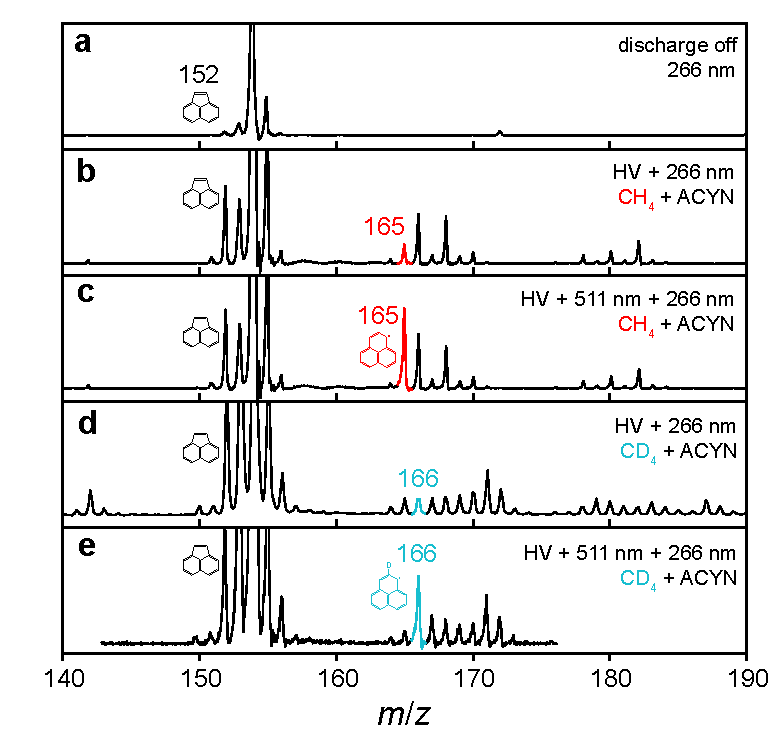
\includegraphics[width=15cm]{Figures/Figure1}
	\caption{Mass spectra of products formed in high voltage (HV) electric discharge containing acenaphthylene and CH$_4$/CD$_4$. The phenalenyl radical (\textit{m/z} 165) is highlighted in red. a) R2PI of ACYN at 266\,nm without electric discharge. b) R2PI of products formed in electric discharge from ACYN + CH$_4$ at 266 nm. c) R2C2PI of products formed in electrical discharge from ACYN + CH$_4$. Excitation laser tuned to transition of phenalenyl at 19560 cm$^{-1}$ (511\,nm) and preceding ionisation laser at 266\,nm by 30\,ns. d) R2PI of products formed in electric discharge from ACYN + CD$_4$ at 266 nm. e) R2C2PI of products formed in electrical discharge from ACYN + CD$_4$. Excitation laser tuned to transition at 19565 cm$^{-1}$ and preceding ionisation laser at 266\,nm by 30 ns. The 1d-phenalenyl radical (\textit{m/z} 166) is highlighted in cyan.}
	\label{fig1}
\end{figure}

Figure 1b shows the mass spectrum from ACYN, with a high voltage (HV) discharge of $-1.05$ kV striking the molecular beam expansion 2\,cm after the pulsed nozzle. Two new groups of ions are generated by the HV discharge between \textit{m/z} 164 – 170 and $m/z$ 178 – 184, respectively. These two groups are subsequently spaced from the parent signal ($m/z$ 152) by 12 – 18\,amu indicating the consecutive net addition of CH$_n$, where $n=0-6$.

The species at $m/z$ 165 is assigned to the phenalenyl radical, C$_{13}$H$_9$, resulting from net CH addition to ACYN. The peak at $m/z$ 166 is assigned to 1H-phenalene, C$_{13}$H$_{10}$~\cite{oco17}. The other significant ion signal in this cluster is at \textit{m/z} 168, which corresponds to the addition of CH$_4$ to ACYN, resulting in a molecular formula of C$_{13}$H$_{12}$. A likely suspect is a species similar to 1H-phenalene but with three individual, peripheral, sp$^3$ carbons. Additional minor peaks at \textit{m/z} 167 and 169 are most likely a combination of $^{13}$C isotopologues (of $m/z$ 166 and 168) and radical species.

To confirm the assignment of $m/z$ 165, a tunable laser pulse was introduced to excite the radicals, preceding the ionizing laser pulse by $\sim$30\,ns. The wavelength of the excitation laser was scanned from $541-476$\,nm to measure the resonant 2-colour 2-photon ionisation (R2C2PI) spectrum for the D$_1 \leftarrow$ D$_0$ transition of the phenalenyl radical. Figure~\ref{fig2} shows a comparison with the R2C2PI spectrum recorded by O’Connor et al~\cite{oco11}. The resonance-enhanced ion signal resulting from the excitation laser being tuned to the wavelength of the strongest vibronic transition is shown in Figure~\ref{fig1}c.

\begin{figure} [h!]
	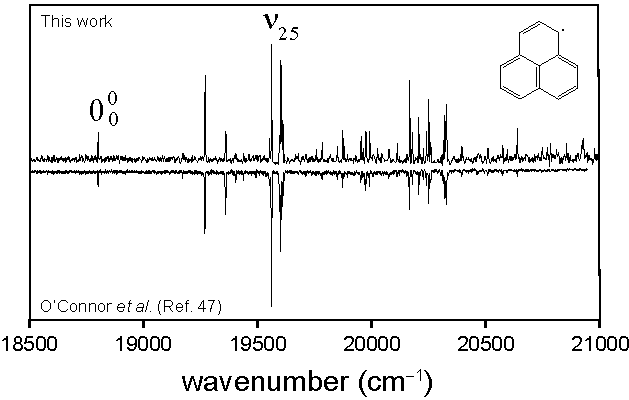
\includegraphics[width=15cm]{Figures/Figure2}
	\caption{Resonant ionisation spectra of the phenalenyl radical (\textit{m/z} 165). Top panel: R2C2PI spectrum recorded in this work (black). Bottom panel: R2C2PI spectrum recorded by O'Connor \textit{et al.}~\cite{oco11} (blue).}
	\label{fig2}
\end{figure}

The formation mechanism of the phenalenyl radical from ACYN was investigated by substituting perdeuterated methane, CD$_4$, into the seeding gas mixture. The resultant mass spectrum from 266\,nm ionization is shown in Figure~\ref{fig1}d. As with the non-deuterated mass spectrum, there are two distinct mass peak clusters produced by CD$_n$ and C$_2$D$_n$ addition to ACYN and ACN.

The wavelength of the excitation laser was scanned around 511\,nm to maximize the $m/z$ 166 signal. The resultant mass spectrum is displayed in Figure~\ref{fig1}e. The resonance enhancement strongly suggests that the \textit{m/z} 166 mass signal corresponds to the d1-phenalenyl radical, C$_{13}$H$_8$D.

To confirm this assignment, the excitation laser was scanned from 535\,nm to 475\,nm. A comparison between the R2C2PI spectra of the phenalenyl radical and the species with \textit{m/z} 166 is shown in Figure~\ref{fig3}. Importantly, no other species produced a vibronic spectrum in this wavelength range. The strong resemblance to the spectrum of the phenalenyl radical confirms the assignment of \textit{m/z} 166 to C$_{13}$H$_8$D. Each peak (cluster) in the deuterated spectrum has been shifted to higher energy by $\sim5$\,cm$^{-1}$ compared to the original spectrum.

It may be tempting to ascribe the splitting of the origin peak at 18800 cm$^{-1}$ to two different deuteration sites: either on or off the C$_2$ axes. However, the D$_1$ state of phenalenyl is a $E''\otimes e'$ Jahn-Teller problem. Briefly, the potential energy component of the Hamiltonian for the $1E''$ state of phenalenyl can be written, in the diabatic basis,
\begin{equation}\label{JT}
  \mathbf{V} = \left[\begin{array}{cc}
                       \lambda\rho^2 - kQ_x + (\delta Q_x) & +kQ_y \\
                       +kQ_y &  \lambda\rho^2 + kQ_x
                     \end{array}
    \right]
\end{equation}
where the rows and columns represent the two components of the degenerate electronic state, $|\mathcal{E}_x\rangle,|\mathcal{E}_y\rangle$. The symbols $Q_x$ and $Q_y$ are the components of a degenerate $e'$ Jahn-Teller active mode, with $\rho^2=Q_x^2+Q_y^2$. The term in parentheses is discussed below. Diagonalization of this matrix ($\delta=0$) generates the familiar Jahn-Teller conical intersection.

With a single deuterium atom in the 2-position ($C_{2v}$), there will be a zero-point energy difference between positive and negative distortions in, say, $Q_x$. This is quantum-induced symmetry-breaking, as observed in dihydroanthracenyl radicals.\cite{kre19} This effect is introduced by augmenting the linear term in at least one of the diagonal matrix elements. This tilts the potential to localize the minimum energy.\cite{lia93} A full account of this effect in asymmetrically deuterated cyclopentadienyl radicals is given in Reference \citenum{lia93}.

In the basis of $|\mathcal{E}_{x,y}\rangle\otimes|v_x,v_y\rangle$ harmonic oscillator wavefunctions, $|\mathcal{E}_{x,y}\rangle\otimes\{|0,0\rangle, |0,1\rangle, |1,0\rangle\}$ which are eigenfunctions of the potential $V = \lambda \rho^2$, with eigenvalues $\{\epsilon_0,\epsilon_1,\epsilon_1\}$
\begin{equation}\label{JT2}
  \mathbf{H} = \left[\begin{array}{cccccc}
                      \epsilon_0 & -k' & 0 & 0 & 0 & +k\\
                      -k' & \epsilon_1 & 0 & 0 & 0 & 0 \\
                      0 & 0 & \epsilon_1 & +k & 0 & 0 \\
                      0 & 0 & +k & \epsilon_0 & +k & 0\\
                      0 & 0 & 0 & +k & \epsilon_1 & 0\\
                      +k & 0 & 0 & 0 & 0 & \epsilon_1 
                     \end{array}
    \right]
\end{equation}

where $\langle1|Q_{x,y}|0\rangle=1$ and $k'=k-\delta$. In the absence of zero-point energy effects, diagonalization of this matrix yields a degenerate ground state. However, the term $\delta$ lifts this degeneracy, resulting in a splitting, consistent with the experimental spectrum presented in Figure \ref{fig3}. An even more complicated pattern than is observed might be expected were there both isotopomers present, in addition to the asymmetric Jahn-Teller effect. A complete assignment of the deuterated spectrum will be provided in a forthcoming publication.

\begin{figure}[h!]
	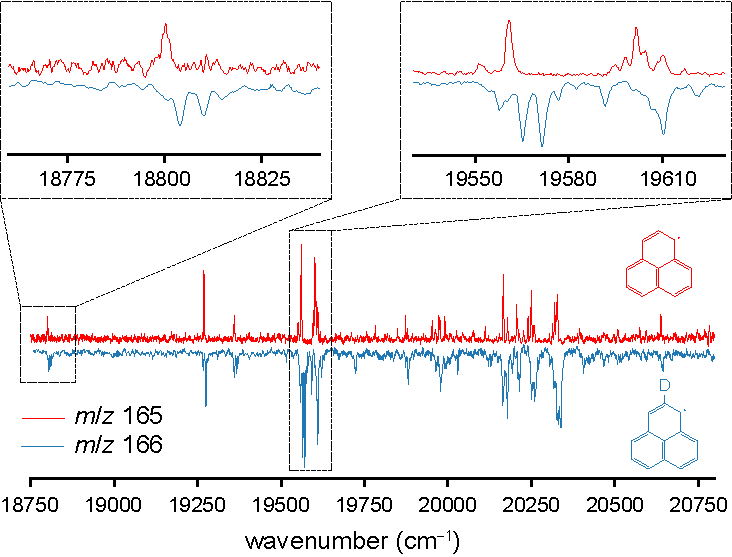
\includegraphics[width=0.85\textwidth]{Figures/Figure3}
	\caption{Top: A comparison of the resonant ionisation spectra of phenalenyl radical (C$_{13}$H$_9$) (red) and deuterated phenalenyl radical (C$_{13}$H$_8$D) (blue). Top left: Origin band. Top right: Most intense bands in the spectrum.}
	\label{fig3}
\end{figure}

This result provides insight into the formation mechanism of phenalenyl radical from ACYN. A mass shift from \textit{m/z} 165 to 166 shows that only a single deuterium atom has been substituted into the phenalenyl radical. This is inconsistent with the methylation mechanism put forth by Porfiriev~\textit{et.}~\textit{al.}~\cite{por20}, in which hydrogen abstraction from ACYN allows for CH$_3$ (CD$_3$) addition to the resultant radical site of the acenaphthyl radical. The methylated product may then follow several different pathways leading to the phenalenyl radical. However, each pathway in their proposed reaction scheme involves two hydrogen (deuterium) atoms from the CH$_3$ (CD$_3$) radical being present in the final product~\cite{por20}. The deuterated reaction scheme for the methylation mechanism is shown in Figure~\ref{fig4}a.

\begin{figure}[h!]
	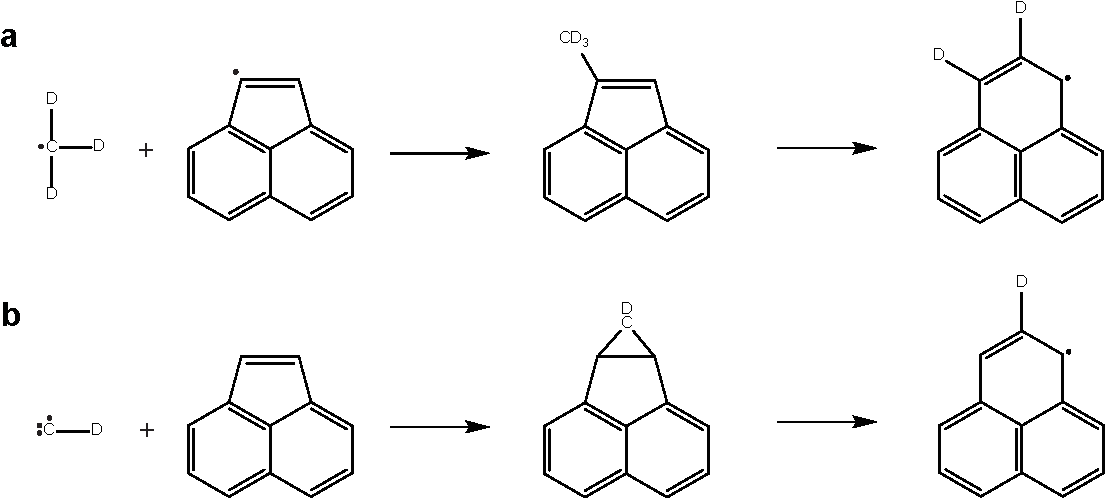
\includegraphics[width=1\textwidth]{Figures/Figure4}
	\caption{ a) Methylation reaction scheme for formation of phenalenyl radical from 1-acenaphthyl radical + CD$_3$$\cdot$, proposed by Porfiriev~\textit{et. al.}~\cite{por20}
		b) Cycloaddition reaction scheme for the formation of phenalenyl radical from acenaphthylene + CD$\cdot$.}
	\label{fig4}
\end{figure}

Results from this work are in agreement with the CH cycloaddition mechanism reported by Trevitt and Goulay~\cite{tre16}, where CH addition across a double bond allows for expansion of the five-membered ring in ACYN to form one of the six-membered rings in phenalenyl. However, this process is also complicated by the potential for CH reaction at the six-membered rings in ACYN, which one might expect to lead to tropyl- and benzyl-like structures. To investigate these aspects of the mechanism, we carried out a computational chemistry investigation.



Figure~\ref{fig5} shows the reaction scheme developed for phenalenyl formation from CH attack on the five-membered ACYN ring. The cycloadduct channel, depicted as the lower pathway, is formed via CH attack across the double bond of the five-membered ring and cuts through multiple pathways to directly form phenalenyl. By tracing the single added hydrogen (deuterium) along this pathway we can deduce it will finish in the 2-position (C$_{2\mathrm{v}}$). CH insertion into the C-H bond of the five-membered ACYN ring may also occur. The resultant intermediate undergoes ring opening chemistry, generating phenalenyl either via a cycloadduct, or by direct insertion into the double bond. Tracing the hydrogen (deuterium) along these pathways results in an ambiguous final position, either on or off the C$_2$ axes. However, as only one isotopomer appears to be present in the experimental spectra presented in Figure~\ref{fig3}, the reaction mechanism must have a propensity to favour one isotopomer over the other, consistent with the cycloaddition mechanism dominating over CH insertion. 


%CH insertion into the C-H bond of the five-membered ACYN ring may also occur. The resultant intermediate undergoes ring opening chemistry, generating phenalenyl either via a cycloadduct, or by direct insertion into the double bond. Tracing the hydrogen (deuterium) along these pathways results in an ambiguous final position,  either on or off the C2 axes. This is contrary to our previous arguments based on the splitting pattern of the origin, and so we believe the reaction mechanism has a propensity to favour one isotopomer over the other. Further work is required to determine which structure dominates. 

%Figure~\ref{fig5} shows the reaction scheme developed for phenalenyl formation from CH attack on the five-membered ACYN ring. Insertion into a C-H bond generates a CH$_{2}$ radical that strikes on the five membered ring of ACYN, followed by a ring opening chemistry generating phenalenyl. The cycloadduct channel, formed via CH attack across the double bond of the five membered ring, cuts through multiple pathways to directly form phenalenyl.

\begin{figure}[h!]
	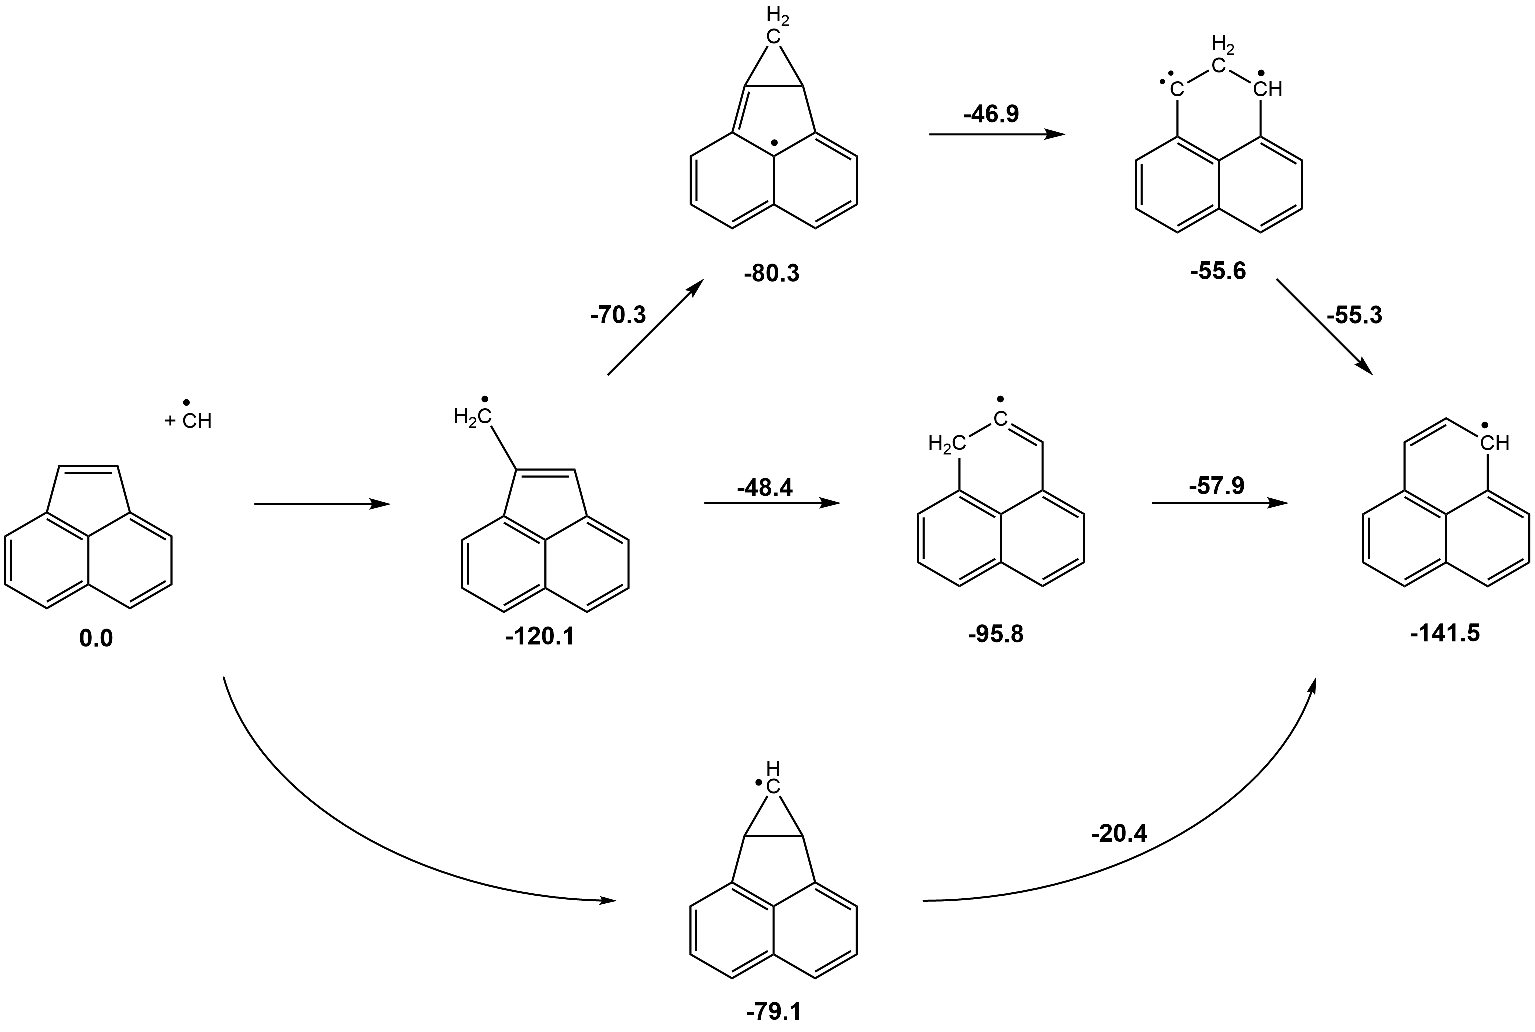
\includegraphics[width=1\textwidth]{Figures/Figure5}
	\caption{Reaction scheme for formation of phenalenyl from a CH attack on the five-membered ACYN ring. Calculations were performed at M06-2X/6-31G(2df,p) and G3X-K level of theory. The energies are in kcal/mol.}
	\label{fig5}
\end{figure}

As mentioned, CH reaction with ACYN may also proceed via attack at a six-membered ring, where cycloaddition and C-H bond insertion are again both available. Figure~\ref{fig6} demonstrates that the cycloaddition process leads to a tropyl-like intermediate structure with no barrier. It may then rearrange to phenalenyl, with all barriers well below entrance. The formed tropyl-like intermediate undergoes an internal H-atom transfer, a rate limiting step in the rearrangement to phenalenyl. Subsequently, a ring formation and cleavage mechanism occurs via a low energy barrier to finally produce phenalenyl. Following the added deuterium atom we see that both pathways depicted in Figure~\ref{fig6} result in a single isotopomer, being the off-axis one. Therefore, cycloaddition must favour attack at either the five-membered or six-membered ring, to account for only one isotopomer being observed in the deuterated spectrum.

The C-H bond insertion mechanism at the six membered ring is somewhat more complex, as there are three unique H atoms, leading to three unique benzyl-like intermediates. One of these three processes is illustrated in Figure~\ref{fig7} with the others presented in the supplementary information. Again, formation of the initial resonantly stabilised radical (RSR) is barrierless and highly exothermic, providing it with significant excess vibrational energy to overcome subsequent barriers to rearrangement. Here this occurs via CH$_2$ attack followed by insertion into the ring at either of the two adjacent carbons. A subsequent H-shift then returns the tropyl-like structure seen before, which will follow on to produce phenalenyl. As with insertion at a C-H on the five membered ring, this process results in scrambling of H and D when CD initiates the reaction. The final isotopomer therefore can not be unique, again leading us to conclude that cycloaddition must be the dominant mechanism. %(interestingly the conventional benzyl - tropyl mechanism is  unavailable because of the fused rings but there is more than enough energy anyway). From here will follow on to phenalenyl.  

\begin{figure}[h!]
	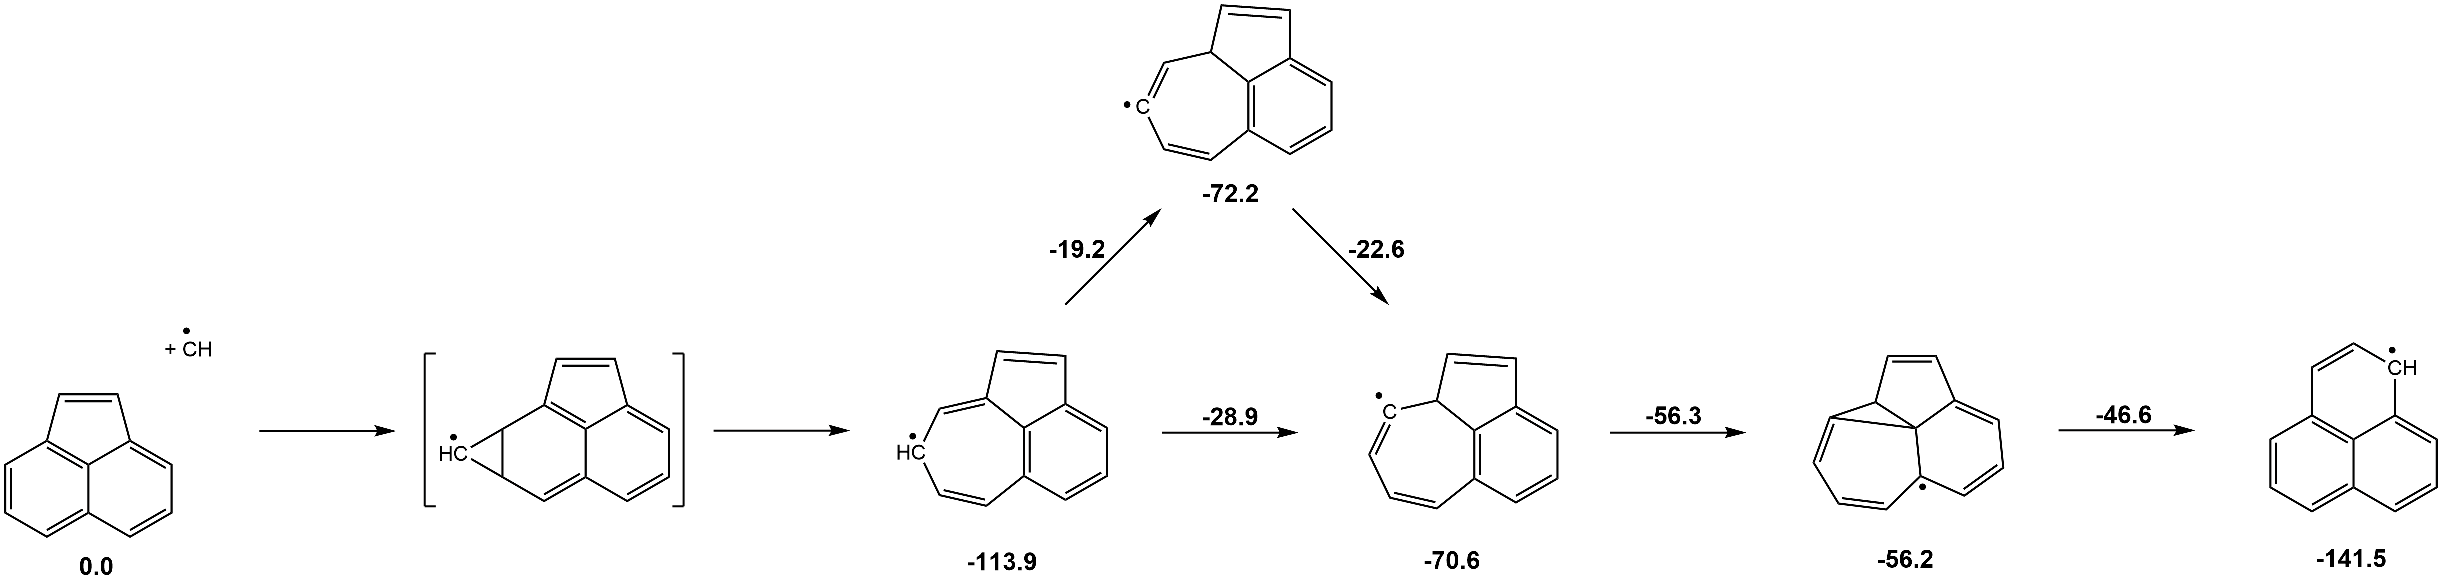
\includegraphics[width=1\textwidth]{Figures/Figure6}
	\caption{Formation of phenalenyl from a CH attack on the 6-membered ACYN ring, via a tropyl-like intermediate RSR. Calculations were performed at M06-2X/6-31G(2df,p) and G3X-K level of theory. The energies are in kcal/mol.}
	\label{fig6}
\end{figure}

\begin{figure}[h!]
	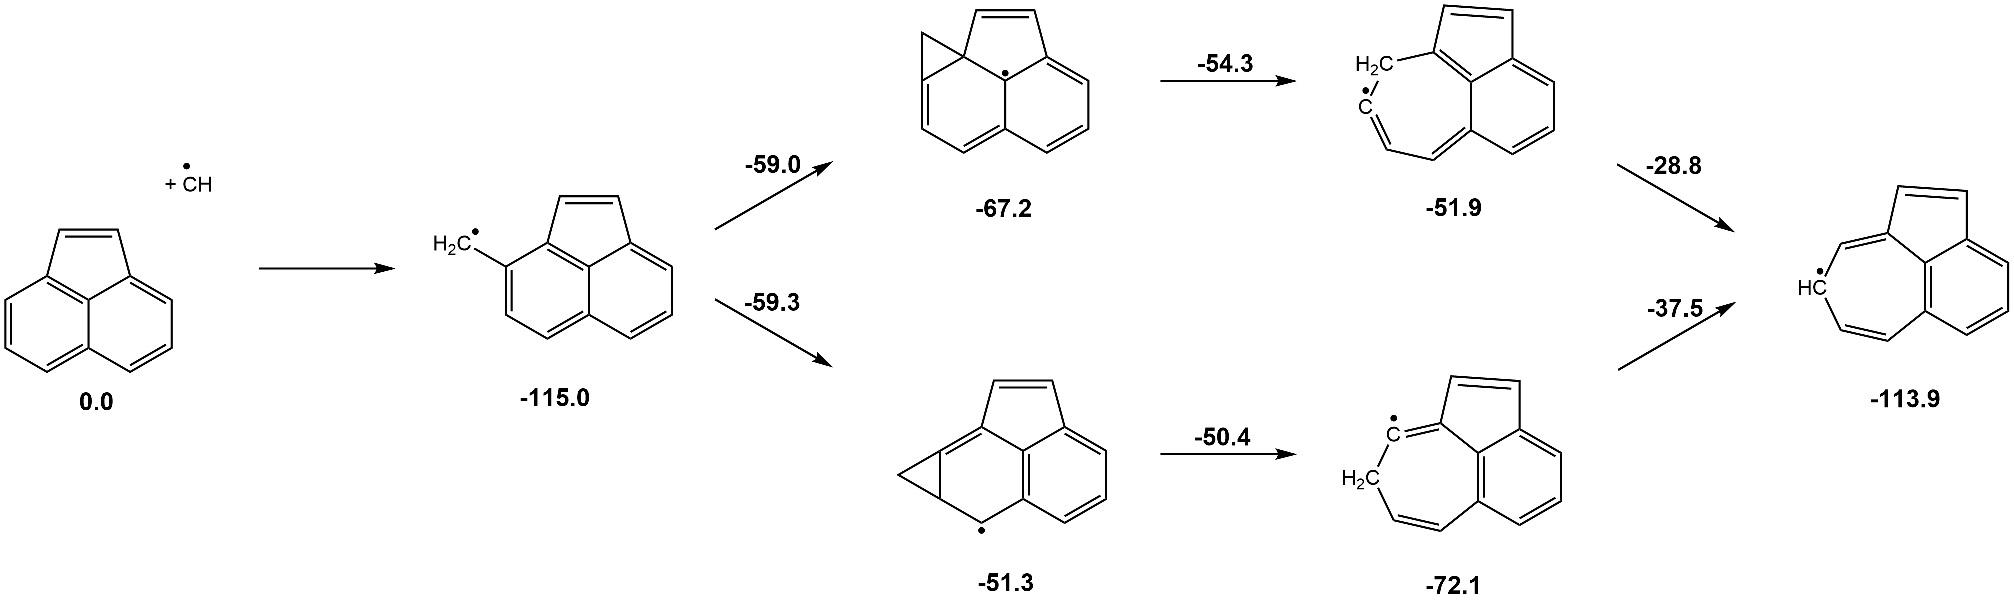
\includegraphics[width=1\textwidth]{Figures/Figure7}
	\caption{Reaction scheme for CH insertion, forming the tropyl-like RSR. Calculations were performed at M06-2X/6-31G(2df,p) and G3X-K level of theory. The energies are in kcal/mol.}
	\label{fig7}
\end{figure}


% Figure~\ref{scheme}b displays the presently hypothesized reaction mechanism for the formation of phenalenyl radical from ACYN. In this reaction, the CH or CD radical is inserted across the $\pi$-bond of the cyclopenta-fused ring of ACYN, forming a bicyclic intermediate. This may then isomerize, resulting in ring opening and the formation of the third six-membered ring. For this scheme, there is no abstraction of the original hydrogens of ACYN and only a single additional hydrogen/deuterium is required to form the phenalenyl radical.

In short, all roads lead to phenalenyl. The most straightforward route is via direct attack at the five-membered ring, and for the CD reaction this produces a single C$_{2\mathrm{v}}$ isotopomer, which is consistent with our spectroscopic analysis. Cycloaddition and insertion at the six-membered rings makes tropyl- and benzyl-like RSRs, but in low pressure and energetic environments they will be able to rearrange to phenalenyl. % we are looking at potential molecular dissociation products that could be spat out in the vacuum of space. Nothing obvious but 150 kcal/mol should be enough to even cleave a H to give a benzyne looking thing.


The CH cycloaddition mechanism working in conjunction with the HACA mechanism is a plausible explanation for the production of the multitude of large, planar PAHs formed in combustion processes. The HACA mechanism will predominantly generate a five-membered ring in the bay region of a PAH. The CH cycloaddition mechanism will then cause ring expansion to form another six-membered ring, and the process can repeat itself. This subsequent combination of mechanisms can account for the formation of PAHs beyond the phenalenyl radical, such as pyrene, cyclopenta[cd]pyrene and the olympicenyl radical. The high concentrations of CH radicals in combustion environments and its detection in the interstellar medium further supports the plausibility of CH cycloaddition as a crucial component of the PAH formation mechanism~\cite{lov11,tin11,zha12,ger10,ada41}.

%\begin{figure}
%	\includegraphics[width=0.3\textwidth]{Figures/deut1}
%	\hspace{2cm}
%	\includegraphics[width=0.3\textwidth]{Figures/deut2}
%	\caption{Structure of deuterated phenaenyl radical in which the deuterium atom is substituted in line or off line with a C$_2$ rotational axis.}
%	\label{fig5}
%\end{figure}



%\begin{scheme}
%	\includegraphics[width=1\textwidth]{Figures/Scheme1.png}
%	\caption{The proposed reaction mechanism for the formation of phenalenyl radical from acenaphthylene and CD$\cdot$.}
%	\label{scheme1}
%\end{scheme}

%\section{Discussion}
%Equations may be written using general LaTeX format, and the same labelling method.
%\begin{equation}
%I(\theta,\epsilon) = \frac{\sigma_{\text{total}}(\epsilon)}{4\pi}[1+\beta(\epsilon)\text{P}_2(\cos\theta)],
%\label{eq:beta}
%\end{equation}
%where $\beta$ in Eq.~(\ref{eq:beta}) is a really cool parameter.

%We can also make tables, like this one, Table~\ref{tab:C2H}.
%\begin{table}
%	\caption{This is my table caption.} \label{tab:C2H}
%	\begin{tabular}{c c c c c}
%		\hline Peak & eBE (cm$^{-1}$) & $v$ (cm$^{-1}$) & $\beta$ & Symmetry \\
%		& & & & \\\hline \hline
%		& 23 591 & -231 & + & $\Sigma^+$
%	\end{tabular}
%\end{table}

\section{Conclusion}

We have shown that the phenalenyl radical is produced as a discharge product of ACYN and methane. Substituting CD$_4$ into the seeding gas mixture indicated that the dominant formation mechanism was CH cycloaddition. Calculations show that this reaction occurs through the insertion of CH across the C$-$C $\pi$-bond of the cyclopenta-fused ring of ACYN, forming a three-membered ring, followed by ring-opening to generate the phenalenyl radical. This contradicts the suggestion that the reaction occurs by methylation~\cite{por20}. The conversion of ACYN to the phenalenyl radical is an example of a five-membered ring expanding to a six-membered ring, which is of importance in combustion and interstellar chemistry, and the abundance of CH supports the proposed mechanism in these environments. The CH cycloaddition mechanism may work in tandem with the HACA mechanism to generate larger PAHs beyond the tricyclic phenalenyl radical.

\section{Experimental Details}

The apparatus used for R2C2PI and R2PI has been described previously in more detail~\cite{rei09}. A sample of ACYN is heated to 85\degree C and seeded in 5 bar of a methane/argon gas mixture(Coregas, 1\% Methane/99\% Argon). The seeded gas mix is expanded into a differentially pumped vacuum chamber through a pulsed discharge nozzle (PDN). A voltage of $-$1.05kV is applied to the outer electrode of the PDN for 100 $\mu$s, resulting in a strike which coincides with the expanding gas pulse.

Methane is incorporated into the backing gas mixture to provide an additional source of CH. The discharge products are cooled through supersonic expansion and the central, coldest section of the molecular beam ($\sim$10K) is passed through a 2\,mm diameter skimmer into a second differentially pumped chamber. The cold molecular beam is probed between two positively charged extraction plates of a Wiley-McLaren-type time-of-flight mass spectrometer (ToF-MS) using R2C2PI spectroscopy.

A Nd:YAG-pumped dye laser is used as an excitation laser to investigate the first electronic excited states of the phenalenyl radical. The excited radicals are subsequently ionized using the fourth harmonic (266\,nm) of a second Nd:YAG laser, pulsing a few tens of nanoseconds after the excitation pulse. The resultant cations are orthogonally accelerated up the length of the ToF-MS and detected by a multichannel plate (MCP) which produces an electronic signal that is displayed on an oscilloscope. Custom-written LabView software is used to record the spectra and a wavemeter is used to calibrate the laser wavelengths.

\section{Computational details}
Quantum chemical computations were performed using Gaussian-16 program~\cite{g16}. M062-X / 6-31G(2df,p) level of theory and G3X-K were utilized to perform geometry optimizations and single point energies respectively. G3X-K predicts energies accurately within 0.6 kcal/mol, appropriate for thermochemical kinetics~\cite{das13}. Frequency computations verified that all stationary points possess zero imaginary frequencies and one for all saddle points. Intrinsic reaction co-ordinate calculations confirm the connectivity of transition states.

\section{Acknowledgements}
This research was funded by the Australian Research Council (DP190103151). TWS is supported by the Australian Research Council Centre of Excellence in Exciton Science (CE170100026).



% Create the reference section using BibTeX:
\bibliography{PhenRad}

%\newpage
%\onecolumn
%\subsection{TOC Graphic}
%\vspace{2ex}
%\begin{center}
%	\includegraphics[width=8.5cm]{Figures/TOC}
%\end{center}


\end{document}
